\def\mytitle{MATRIX ANALYSIS USING PYTHON}
\def\myauthor{Akana Sai Kumar}
\def\contact{19pa1a0405@vishnu.edu.in}
\def\mymodule{Future Wireless Communication (FWC)}
\documentclass[10pt, a4paper]{article}
\usepackage[a4paper,outer=1.5cm,inner=1.5cm,top=1.75cm,bottom=1.5cm]{geometry}
\twocolumn
\usepackage{graphicx}
\graphicspath{{./images/}}
\usepackage[colorlinks,linkcolor={black},citecolor={blue!80!black},urlcolor={blue!80!black}]{hyperref}
\usepackage[parfill]{parskip}
\usepackage{lmodern}
\usepackage{tikz}
\usepackage{physics}
%\documentclass[tikz, border=2mm]{standalone}
%\usepackage{karnaugh-map}
%\documentclass{article}
\usepackage{tabularx}
%\usepackage{circuitikz}
\usepackage{enumitem}
\usetikzlibrary{calc}
\usepackage{amsmath}
\usepackage{amssymb}
\renewcommand*\familydefault{\sfdefault}
\usepackage{watermark}
\usepackage{lipsum}
\usepackage{xcolor}
\usepackage{listings}
\usepackage{float}
\usepackage{titlesec}
\providecommand{\mtx}[1]{\mathbf{#1}}
\titlespacing{\subsection}{1pt}{\parskip}{3pt}
\titlespacing{\subsubsection}{0pt}{\parskip}{-\parskip}
\titlespacing{\paragraph}{0pt}{\parskip}{\parskip}
\providecommand{\qfunc}[1]{\ensuremath{Q\left(#1\right)}}
\providecommand{\sbrak}[1]{\ensuremath{{}\left[#1\right]}}
\providecommand{\lsbrak}[1]{\ensuremath{{}\left[#1\right.}}
\providecommand{\rsbrak}[1]{\ensuremath{{}\left.#1\right]}}
\providecommand{\brak}[1]{\ensuremath{\left(#1\right)}}
\providecommand{\lbrak}[1]{\ensuremath{\left(#1\right.}}
\providecommand{\rbrak}[1]{\ensuremath{\left.#1\right)}}
\providecommand{\cbrak}[1]{\ensuremath{\left\{#1\right\}}}
\providecommand{\lcbrak}[1]{\ensuremath{\left\{#1\right.}}
\providecommand{\rcbrak}[1]{\ensuremath{\left.#1\right\}}}
\newcommand{\figuremacro}[5]{
    \begin{figure}[#1]
        \centering
        \includegraphics[width=#5\columnwidth]{#2}
        \caption[#3]{\textbf{#3}#4}
        \label{fig:#2}
    \end{figure}
}
\newcommand{\myvec}[1]{\ensuremath{\begin{pmatrix}#1\end{pmatrix}}}
\let\vec\mathbf
\lstset{
frame=single, 
breaklines=true,
columns=fullflexible
}

\title{\mytitle}
\author{\myauthor\hspace{1em}\\\contact\\FWC22032\hspace{6.5em}IITH\hspace{0.5em}\mymodule\hspace{6em}Assignment}
\begin{document}
	\maketitle
	\tableofcontents
   \section{Problem}
The foci of the ellipse $\frac{x^2}{16}$+$\frac{y^2}{b^2}$=1 and the hyperbola $\frac{x^2}{144}$-$\frac{y^2}{81}$=$\frac{1}{25}$ coincide . Then 
the value of   $b^2$
   
 %The area of the quadrilateral formed by the tangents at the end points of latus rectum to the ellipse \begin{align}
%\frac{x^2}{9}+\frac{y^2}{5}=1
 % \end{align}
\section{Construction}
  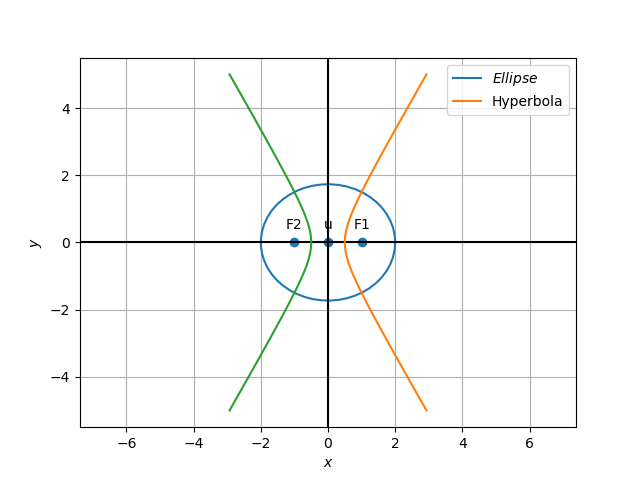
\includegraphics[scale=0.47]{conic1.png}
  	\begin{center}
  Figure of construction
  	\end{center}
  \section{Solution}

Hyperbola equation : \begin{align}
\frac{x^2}{144}-\frac{y^2}{81}=\frac{1}{25}
  \end{align}
The standard equation of the conics is given as :
\begin{align}
\vec{x}^{\top}\vec{V}\vec{x}+2\vec{u}^{\top}\vec{x}+f=0
\end{align}

The given ellipse can be expressed as conics with \\parameters
\begin{align}
	\lambda_1&=25/144,\lambda_2=-25/81 \\ \vec{V} &= \myvec{	\lambda_1& 0 \\
			          0 & \lambda_2}  
		    , \vec{u} = \myvec{0 \\0}, f = -1
	\end{align}
	Eccentricity:
	\begin{align}
	 e&=\sqrt{1-\frac{\lambda_1}{\lambda_2}}\\
	 \implies e&=15/12
	 \end{align}
	 Foci:
	 \begin{align}
	 f0&=-f,\vec{e}_1 = \myvec{1 \\0}\\
	 %\vec{F}&= \pm e\sqrt{\frac{\abs{f_0}}{\lambda_2\brak{1-e^2}}}\\
	 	 \vec{F}_1&=  e\sqrt{\frac{\abs{f_0}}{\lambda_2\brak{1-e^2}}}\vec{e}_1\\
	 	 \vec{F}_2&= - e\sqrt{\frac{\abs{f_0}}{\lambda_2\brak{1-e^2}}}\vec{e}_1\\
	 \implies \vec{F}_1&=\myvec{3\\0},\vec{F}_2=\myvec{-3\\0}
	 \end{align}
	 
Ellipse equation : \begin{align}
\frac{x^2}{16}+\frac{y^2}{b^2}=1
  \end{align}
The standard equation of the conics is given as :
\begin{align}
\vec{x}^{\top}\vec{V}_1\vec{x}+2\vec{u}^{\top}_1\vec{x}+f_1=0
\end{align}
	 The given ellipse can be expressed as conics with \\parameters
\begin{align}
	\lambda_3&=b^2,\lambda_4=16 \\ \vec{V}_1 &= \myvec{	\lambda_3& 0 \\
			          0 & \lambda_4}  
		    , \vec{u}_1 = \myvec{0 \\0}, f_1 = -16b^2
	\end{align}
	Eccentricity:
	\begin{equation}
	 e =\sqrt{1-\frac{\lambda_3}{\lambda_4}}\\
	 \end{equation}
	 \begin{equation}
	 e =\sqrt{1-\frac{b^2}{16}}\\
	 \end{equation}
	 Foci:
	 \begin{align}
	 f_0&=-f_1,\vec{e}_1 = \myvec{1 \\0}\\
	% \vec{F}_3&= \pm e\sqrt{\frac{\abs{f_0}}{\lambda_4\brak{1-e^2}}}\\
	 	 \vec{F}_4&=  e\sqrt{\frac{\abs{f_0}}{\lambda_4\brak{1-e^2}}}\vec{e}_1\\
	 	 \vec{F}_5&= - e\sqrt{\frac{\abs{f_0}}{\lambda_4\brak{1-e^2}}}\vec{e}_1	 	 
	 \end{align}
Then equate the $\vec{F}_1$ =$\vec{F}_4$we get the $b^2$ \\
\begin{align}
	b^2 = \lambda_4 - (\vec{F}_1^T\vec{e}_1)^2
\end{align}

\end{document}
